\section{Setup and Usage of the Present Work for Theorema Document Processing} \label{usage}

The overview of the package-output of this projects follows Figure \ref{fig:Tma2Tex-Logic-and-Package}, explored in some detail in Chapter \ref{cha:Concept} as far as the concept for the functionality goes. Of interest now is the external view of the package, with two client functions, convertToLatexDoc[] and convertToLatexAndPdfDocs[].

\begin{figure}[h]
    \centering
    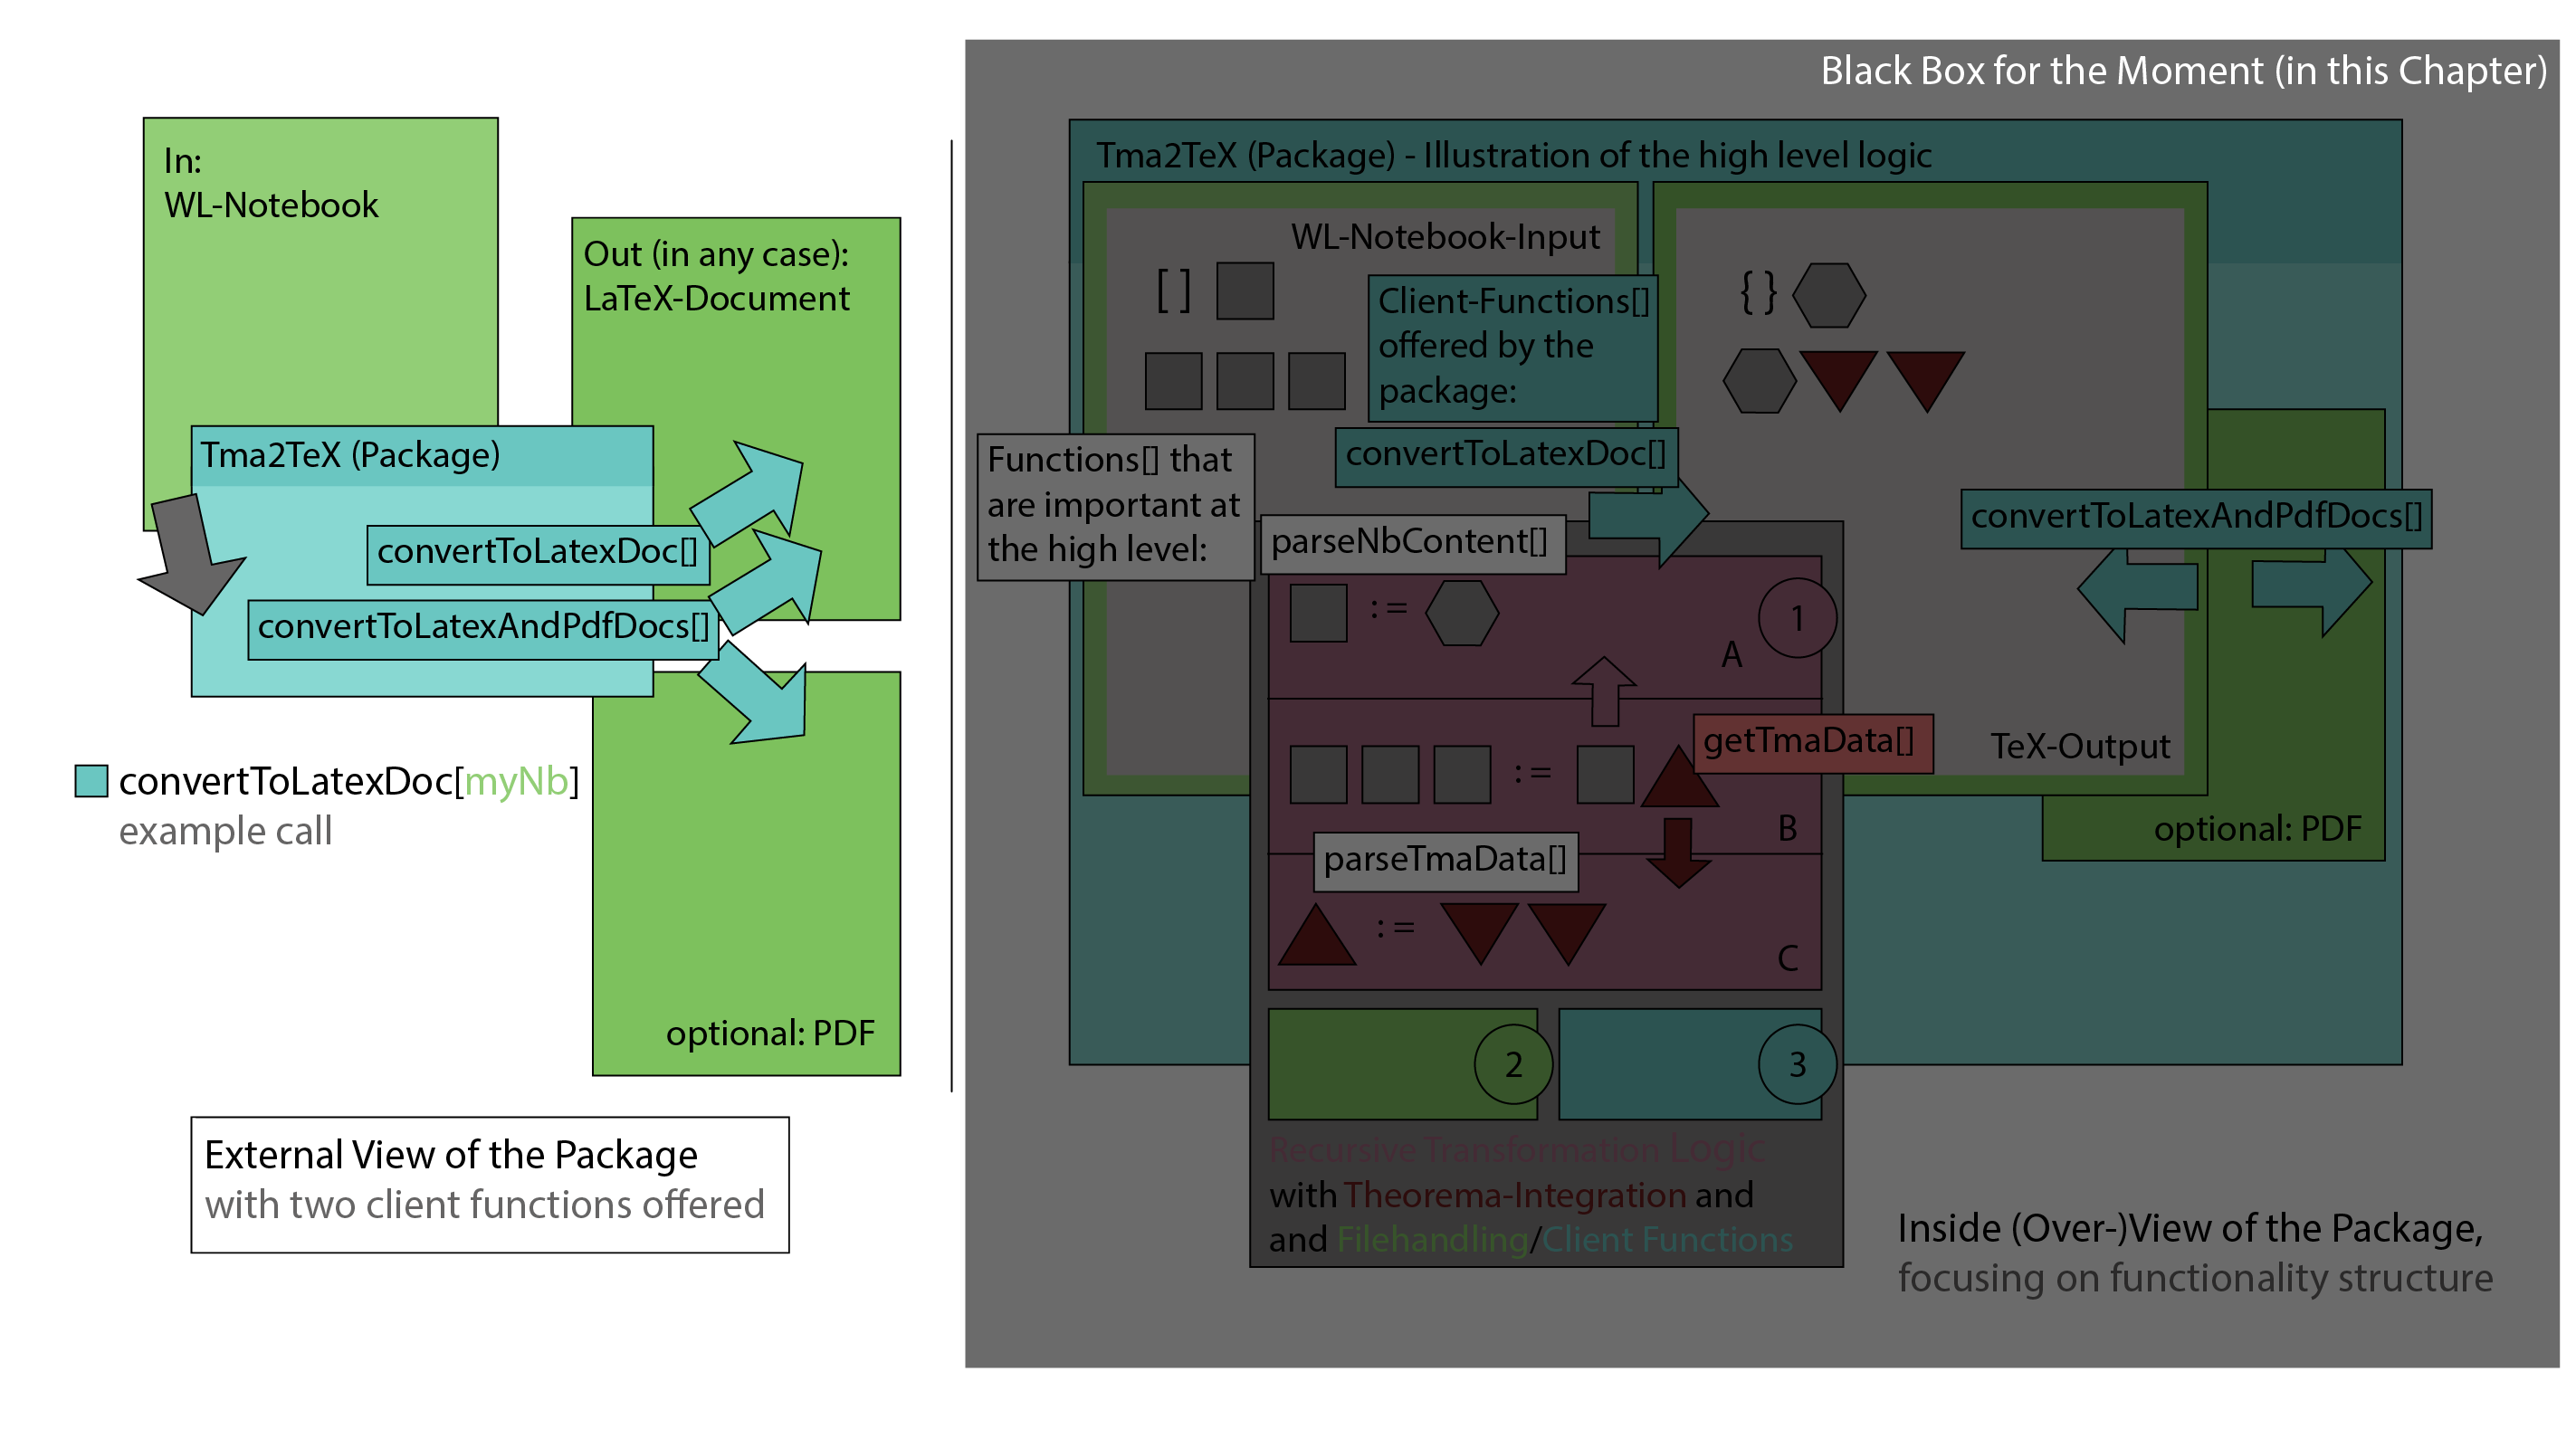
\includegraphics[scale=0.3]{images/introduction/Tma2Tex-Logic-Xt-View-01.png}
    \caption{The client functions convertToLatexDoc[] and convertToLatexAndPdfDocs[] are marked light blue in the above: of interest now is the view on the right, the outside-package view, where the inside will be explored in Chapter \ref{cha:Concept}, putting the client functions into context with the other high-level (programming paradigm) functions involved.}
    \label{fig:Tma2Tex-Logic-and-Package}
\end{figure}

\subsection{Practical/Quick Guide}

What follows is a quick practical guide for setup of this project on any machine with a Mathematica Desktop installation (Mac, Windows, or Linux). 

\subsubsection{Loading Theorema and Tma2tex (as Packages)}

The main dependency is, of course, Theorema, downloadable at the RISC website \cite{noauthor_download_nodate} (name, affiliation and email address are required). The Theorema code is available on GitHub \cite{noauthor_github_nodate} and finally, there is a Programmer Guide  \cite{noauthor_programmers_nodate} available for anyone interested in work on Theorema directly, using tools like Wolfram Workbech \cite{noauthor_wolfram_nodate} as a development environment.

For simple setup for use in Mathematica however, simply move the downloaded and decompressed Theorema package to your preferred location and append this location to the \lstinline+$Path+-variable in Mathematica, so the kernel knows where to find the relevant package (same name with ending ".m" or ".wl" by convention). Similarly, place the Tma2TeX package file ("tma2tex.wl") submitted with this thesis in the same directory (one for all third party packages, otherwise another preferred location of your choosing). Now the  WL-code in Program \ref{loadTmaAndTma2Tex} should be runnable without messaging in a fresh Mathematica notebook. 

\begin{program}
\caption{To load Theorema and Tma2TeX as two packages in a fresh Mathematica notebook, enter this code in a cell and evaluate (shift-enter key combination).}
\label{loadTmaAndTma2Tex}
\begin{LaTeXCode}
(* check $Path if needed, maybe Theorema is already present, but otherwise: *)
tmaDir="C:\\Windows\\path\\to\\Theorema\\package\\file";
AppendTo[$Path, tmaDir];
<<Theorema` 
(* similarly for Tma2tex: *)
tma2texDir="C:\\Windows\\path\\to\\Tma2tex\\package\\file";
AppendTo[$Path, tma2texDir];
<<Tma2tex` 
\end{LaTeXCode}
\end{program}

The setup code loading the two packages is the minimally required code to get this project working.

To actually perform a document transformation, a Theorema notebook like FirstTour.nb included with this project is needed. The notebook can be placed anywhere, but the path will be needed to make the function call.

One more directory location is needed: it is the template directory, called "res" for resources for example, and including the sample template included with this project ("res/tmaTemplate.tex"). Any \LaTeX-Template (which does, however, need to include the relevant \LaTeX-commands for Tma2TeX-specific output, as in the template, and for Tma2TeX to make sensible transformations) may be used. The resources-path held by Tma2TeX can be checked at any time by evaluating \lstinline+Tma2tex`$resDir$+ from the notebook. A full sample notebook, tma2tex.nb, included with this project, implements this call structure. It performs a transformation, placing output files (\LaTeX and PDF in this case) in the same directory held by the variable \lstinline+tma2texDir+.

As a note, if you have any package installed and want to know the file location, you can use \lstinline+FindFile["Theorema`"]+ to find Theorema for example. Note the \lstinline+`+ (backtick) context level delimiter in the package specifications, a WL convention.

\subsubsection{Evaluating a Theorema Notebook in a Tma2tex-Kernel-Session for Theorema-Data-Access}

\lstinline+Theorema`Common`$tmaEnv+ is already mentioned in Program \ref{tma2texFullSample} (and tma2tex.nb): It is the crucial Theorema variable whose content is imported to Tma2TeX and inserted to the output documents according to the relevant Theorema notebook's structure. If an evaluation returns an empty list, it is not loaded. To load it, the best option is to select from the File menu the option "Open ..." and select the desired Theorema notebook (e.g. FirstTour.nb) this way, where the goal is to evaluate the notebook using the same kernel session as the caller notebook, tma2tex.nb in this case, such that the Theorema variables are available to Tma2TeX and filled with the data Theorema provides.

